% Make nice A4 pages for print:
%\usepackage{pgfpages}
%\pgfpagesuselayout{resize to}[a4paper,border shrink=5mm,landscape]

\beamertemplatenavigationsymbolsempty

\setbeamertemplate{bibliography item}[text]

\usepackage[type={CC},modifier={by-sa},version={4.0}]{doclicense}

\usepackage[utf8]{inputenc}
\usepackage{hyperref}
\usepackage{breakurl}
\usepackage{graphicx}
\usepackage{pgfplots}
\usepackage{pgf}
\usepackage{tikz}
\usetikzlibrary{positioning}
\usetikzlibrary{arrows}
\usetikzlibrary{decorations.markings}
\usetikzlibrary{calc}
\usetikzlibrary{matrix}
\usetikzlibrary{shapes}
\usetikzlibrary{decorations.pathmorphing}
\usetikzlibrary{fit}
\usetikzlibrary{backgrounds}
\usetikzlibrary{plotmarks}
\usepackage{stmaryrd}
\usepackage{listings}
\usepackage{pdflscape}
\usepackage{perpage}
\usepackage{appendixnumberbeamer}

%\usepackage[thmmarks,amsmath,amsthm]{ntheorem} % already included in beamer
\usepackage{thm-restate}

\usepackage[sort&compress,numbers]{natbib}  % to be have \citet, \citeauthor, \citeyear

\MakePerPage{footnote}

\tikzstyle{o}=[r,ppBlue]
\tikzstyle{r}=[thick,rectangle,align=center]
\tikzstyle{t}=[r,ppTrans] %,font=\bfseries]
\tikzstyle{dd}=[densely dashed]
\tikzstyle{n}=[r,ppBlue]
\tikzstyle{p}=[r,ppRed]
\tikzstyle{ppRed}  =[draw=red,  fill=  red!20]
\tikzstyle{ppBlue} =[draw=blue, fill= blue!20]
\tikzstyle{ppGreen}=[draw=green,fill=green!20]
\tikzstyle{ppTrans}=[draw=none, fill=none]

\usetheme{Warsaw}

\useoutertheme[subsection=true]{smoothbars}
%\useoutertheme[subsection=false]{miniframes}

\definecolor{bblue}{HTML}{D7DF01}	% yellow-ish actually, for better black/white printing
\definecolor{rred}{HTML}{C0504D}
\definecolor{ggreen}{HTML}{9BBB59}
\definecolor{ppurple}{HTML}{9F4C7C}
\definecolor{lightgray}{rgb}{0.3,0.3,0.3}
\definecolor{lightergray}{rgb}{0.9,0.9,0.9}
\definecolor{UniBlue}{RGB}{83,121,170}

\DeclareTextFontCommand\textintro{\normalfont\bfseries\itshape} % nice!
\newcommand{\intro}[2][]
{%
	\textintro{#2}%
}
\newcommand{\empha}[2][]
{%
	\emph{#2}%
}

%\theoremstyle{plain}
\newcounter{reqcounter}
\newtheorem{requirement}[reqcounter]{Requirement}

%setbeamercolor{structure}{fg=violet}

\makeatletter
\def\th@task{%
    \normalfont % body font
    \setbeamercolor{block title example}{bg=orange,fg=white}
    \setbeamercolor{block body example}{bg=orange!20,fg=black}
    \def\inserttheoremblockenv{exampleblock}
  }
\makeatother

\theoremstyle{task}
\newtheorem{task}{Task}

\newenvironment{assignment}%
{%\setbeamercolor{background canvas}{bg=violet}%
%\setbeamercolor{structure}{fg=cyan!90!black}%
 \setbeamercolor{frametitle}{bg=orange,fg=white}
\begin{frame}}%
{\end{frame}}%

\AtBeginSection[]{
  \begin{frame}
  \vfill
  \centering
  \begin{beamercolorbox}[sep=8pt,center,shadow=true,rounded=true]{title}
    \usebeamerfont{title}\insertsectionhead\par%
  \end{beamercolorbox}
  \tableofcontents
  \vfill
  \end{frame}
}




\pgfplotsset{compat=1.14}
\author{Markus Raab}


\date{08.05.2018}

\begin{document}

\renewcommand{\enquote}[1]{\emph{``#1''}} % Cannot be done earlier

%%%%%%%%%%%%%%%%%%%%%%%%%%%%%%%
\begin{frame}
	\titlepage
	\doclicenseThis
\end{frame}


\begin{frame}
	Lecture is every week Wednesday 09:00 - 11:00.

	\begin{description}
		\item[06.03.2019:] {\color{gray}topic, teams}
		\item[13.03.2019:] {\color{gray}TISS registration, initial PR}
		\item[20.03.2019:] {\color{gray}other registrations, guest lecture}
		\item[27.03.2019:] {\color{gray}PR for first issue done, second started}
		\item[03.04.2019:] {\color{gray}first issue done, PR for second}
		\item[10.04.2019:] {\color{gray}mid-term submission of exercises}
		\item[08.05.2019:] {\color{red}different location: Complang Libary}
		\item[15.05.2019:]
		\item[22.05.2019:] all 5 issues done
		\item[29.05.2019:]
		\item[05.06.2019:] final submission of exercises
		\item[12.06.2019:]
		\item[19.06.2019:] last corrections of exercises
		\item[26.06.2019:] exam
	\end{description}
\end{frame}

\begin{assignment}
	\frametitle{Tasks for today}
	(until 08.05.2019 23:59)
	
	\begin{task}
	Incorporate feedback for teamwork and homework.
	\end{task}

	\begin{task}
	Third PR done, PR for fourth issue created and write some text in your last issue (if 5 issues are not yet assigned to you).
	\end{task}
\end{assignment}

\begin{assignment}
	\frametitle{Tasks for next week}
	(until 15.05.2019 23:59)

	\begin{task}
	Fourth PR done, PR for fifth issue created.
	\end{task}

	\begin{task}
	Continue teamwork and homework.
	\end{task}
\end{assignment}

\begin{frame}
	\frametitle{Popular Topics}
	\vspace{-0.55cm}
	\setlength{\columnsep}{-1.3cm}
	\raggedright
	\begin{multicols}{2}
	\begin{description}
	\item[14] tools
	\item[9] testability
	\item[9] {\color{red} code-generation}
	\item[7] context-awareness
	\item[6] {\color{red} specification}
	\item[6] misconfiguration
	\item[6] {\color{gray} complexity reduction}
	\item[5] validation
	\item[5] points in time % (early detection)
	\item[5] error messages
	\item[5] {\color{gray} auto-detection}
	\item[4] user interface
	\item[4] {\color{red} introspection}
	\item[4] design
	\item[4] cascading
	\item[4] {\color{red} architecture of access}
	\item[3] {\color{gray} configuration sources}
	\item[3] {\color{gray} config-less systems}
	\item[2] secure conf
	\item[2] {\color{gray} architectural decisions}
	\item[1] push vs.\ pull
	\item[1] infrastructure as code
	\item[1] full vs.\ partial
	\item[1] convention over conf %iguration
	\item[1] CI/CD
	\item[0] documentation
	\end{description}
	\end{multicols}
\end{frame}

\begin{frame}
	\frametitle{Metalevels (Recapitulation)}
	\begin{alertblock}{Question}
	Describe the three Metalevels in Elektra.
	\end{alertblock}

	\pause
	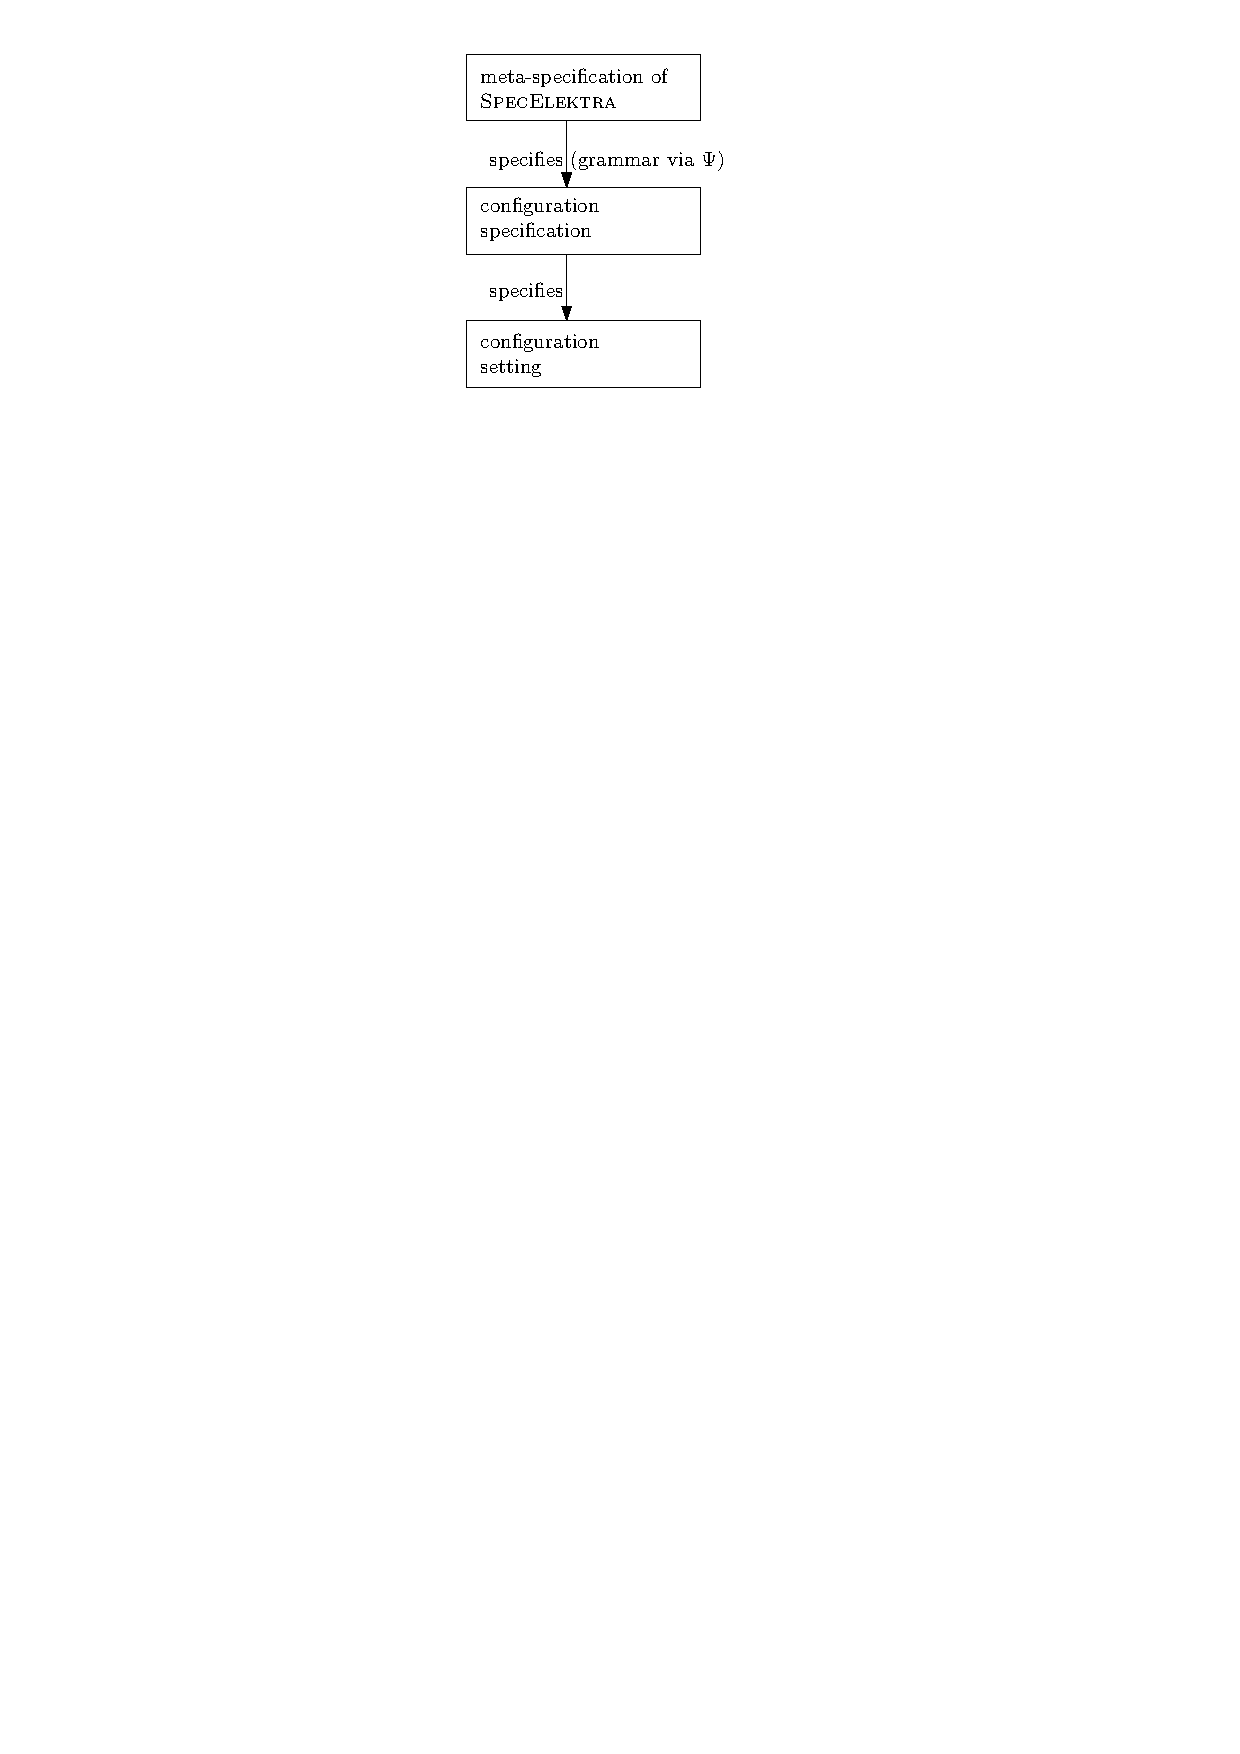
\includegraphics{metalevels}
\end{frame}

\begin{frame}
	\frametitle{SpecElektra (Recapitulation)}
	\pause

	\fontsize{18}{0}\selectfont
	\ExecuteMetaData[../book/approach.tex]{definition-spec}
\end{frame}

\begin{frame}
	\frametitle{Recapitulation (Requirements of SpecElektra)}

	\pause
	\begin{itemize}
	\item formal and informal
	\item should strive for completeness
	\item should be extensible
	\item should be external to application
	\item open for introspection (for tooling)
	\item should talk to users
	\item should allow generation of artefacts
	\end{itemize}
\end{frame}

\begin{frame}
	\frametitle{Modularity (Recapitulation)}
	\pause
	\Large
	\ExecuteMetaData[../book/backend.tex]{definition-modularity}
\end{frame}

\begin{frame}
	\frametitle{Vertical Modularity (Recapitulation)}
	\begin{alertblock}{Question}
	Explain the content of the figure.
	\end{alertblock}
	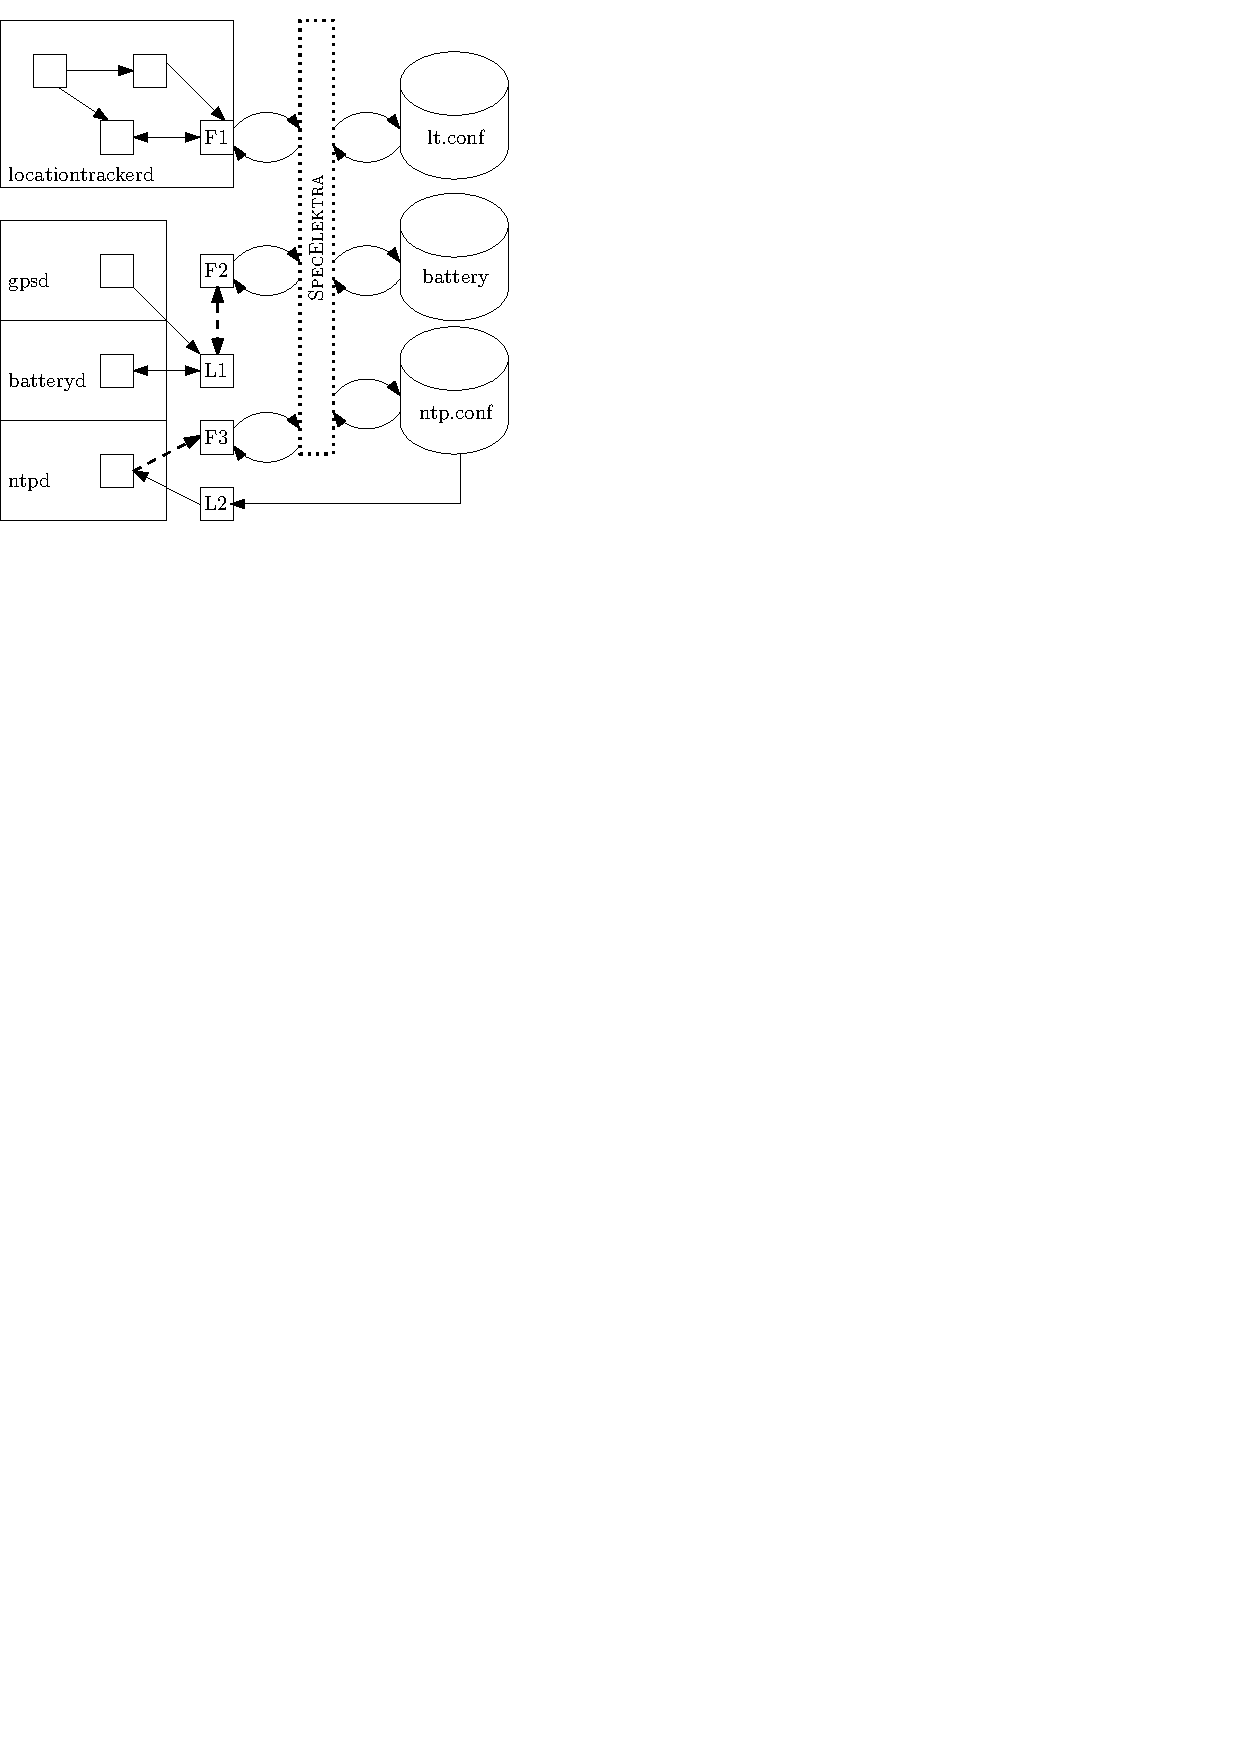
\includegraphics[scale=0.7]{verticalmodularity}
\end{frame}

\begin{frame}
	\frametitle{Plugins (Recapitulation)}
	\pause
	\Large
	\ExecuteMetaData[../book/approach.tex]{definition-plugins}
\end{frame}

\begin{frame}
	\frametitle{Introspection (Recapitulation)}
	\pause
	\begin{itemize}
	\item unified get/set access to (meta*)-key/values
	\item access via applications, CLI, GUI, web-UI, ...
	\item access via any programming language (similar to file systems)
	\item GUI, web-UI can semantically interpret metadata
	\end{itemize}
\end{frame}


\begin{frame}
	\frametitle{Goals for today}
	\textit{learning outcome:}
	\begin{itemize}
	\item evaluate a configuration system and decide about use of
	\begin{itemize}
	\item code generation
	\item system-wide introspection
	\end{itemize}
	\end{itemize}
\end{frame}
%%%%%%%%%%%%%%%%%%%%%%%%%%%%%%%%%%%%%%%%%% 

\section{Code Generation}

\subsection{Why?}

\begin{assignment}
	\begin{task}
	How to ensure that configuration access points match with present configuration settings?
	\end{task}
\end{assignment}

\begin{frame}
	\frametitle{Rationale (Partly Recapitulation)}
	Configuration Specification:
	\begin{itemize}
	\item without specification you and others do not even know which settings are available
	\item needed for any further techniques we will discuss:
		\begin{itemize}
		\color{red}
		\item code generation guarantees that configuration access points match with specification
		\item validation guarantees that configuration settings match with specification
		\end{itemize}
	\item essential for \intro[no-futz computing]{no-futz computing}~\citet{holland2001nofutz}
	\item the foundation for any advanced tooling like configuration management tools
	\item needed as communication of producers and consumers of configuration
	\end{itemize}
\end{frame}

\begin{frame}[fragile]
	\frametitle{Current Challenges}
	Configuration access code usually has:
	\pause
	\begin{itemize}
	\item code duplications and unsafe APIs
	\item hard-coded default values
	\item unexpected transformations (e.g., truncating of values)
	\item inconsistencies (e.g., case sensitivity)
	\item no introspection facilities (which keys and values are allowed?)
	\end{itemize}
	\begin{example}[Silent Overruling \cite{xu2013blame}]
	\begin{code}[gobble=4,language=C++]
	if (!strcasecmp(token, "on")) {
		*var = 1;
	} else {
		*var = 0;
	} /* src/cache_cf.cc from Squid */
	\end{code}\end{example}
\end{frame}

\begin{frame}[fragile]
	\frametitle{Real-world example}
	PostgreSQL\footnote{\url{http://doxygen.postgresql.org/guc_8c_source.html}} has following duplications for its configuration settings:
	\begin{itemize}
	\item a global variable and an option record (struct)
	\item an entry in an example (postgresql.conf.sample)
	\item documentation in sgml
	\item in the source code of utils (in-source dump utils, and dozens of external configuration management tools)
	\end{itemize}
	\pause
	\vspace{1em}
	Note: PostgreSQL has a clean implementation, and above list only shows limitations of systems without code generation.
\end{frame}

\begin{assignment}
	\begin{task}
	Brainstorming: Which artefacts can we produce with (code) generation?
	\end{task}
\end{assignment}

\begin{frame}
	Artefacts:
	\begin{itemize}
	\item examples (e.g., defaults)
	\item documentation
	\item auto-completion/syntax highlighting/IDE support
	\item tooling (GUI, Web UI)
	\item validation code
	\item configuration management tool code
	\item configuration access APIs
	\end{itemize}
\end{frame}

\begin{frame}
	\frametitle{Goal}

	\begin{goal}
	Configuration settings should adhere the specification from source to destination.
	\end{goal}

	\begin{restatable}{requirement}{reqGeneration}
	The specification must enable code generation and inconsistencies must be ruled out during compilation.
	\end{restatable}
\end{frame}


\subsection{How?}

\begin{frame}
	\frametitle{Code Generation}

	\ExecuteMetaData[../book/approach.tex]{code-generation}

	\pause
	\vspace{2em}
	But how?
\end{frame}

\begin{frame}
	\frametitle{KeySet (Recapitulation)}

	The common data structure between plugins:
	\vspace{1cm}

	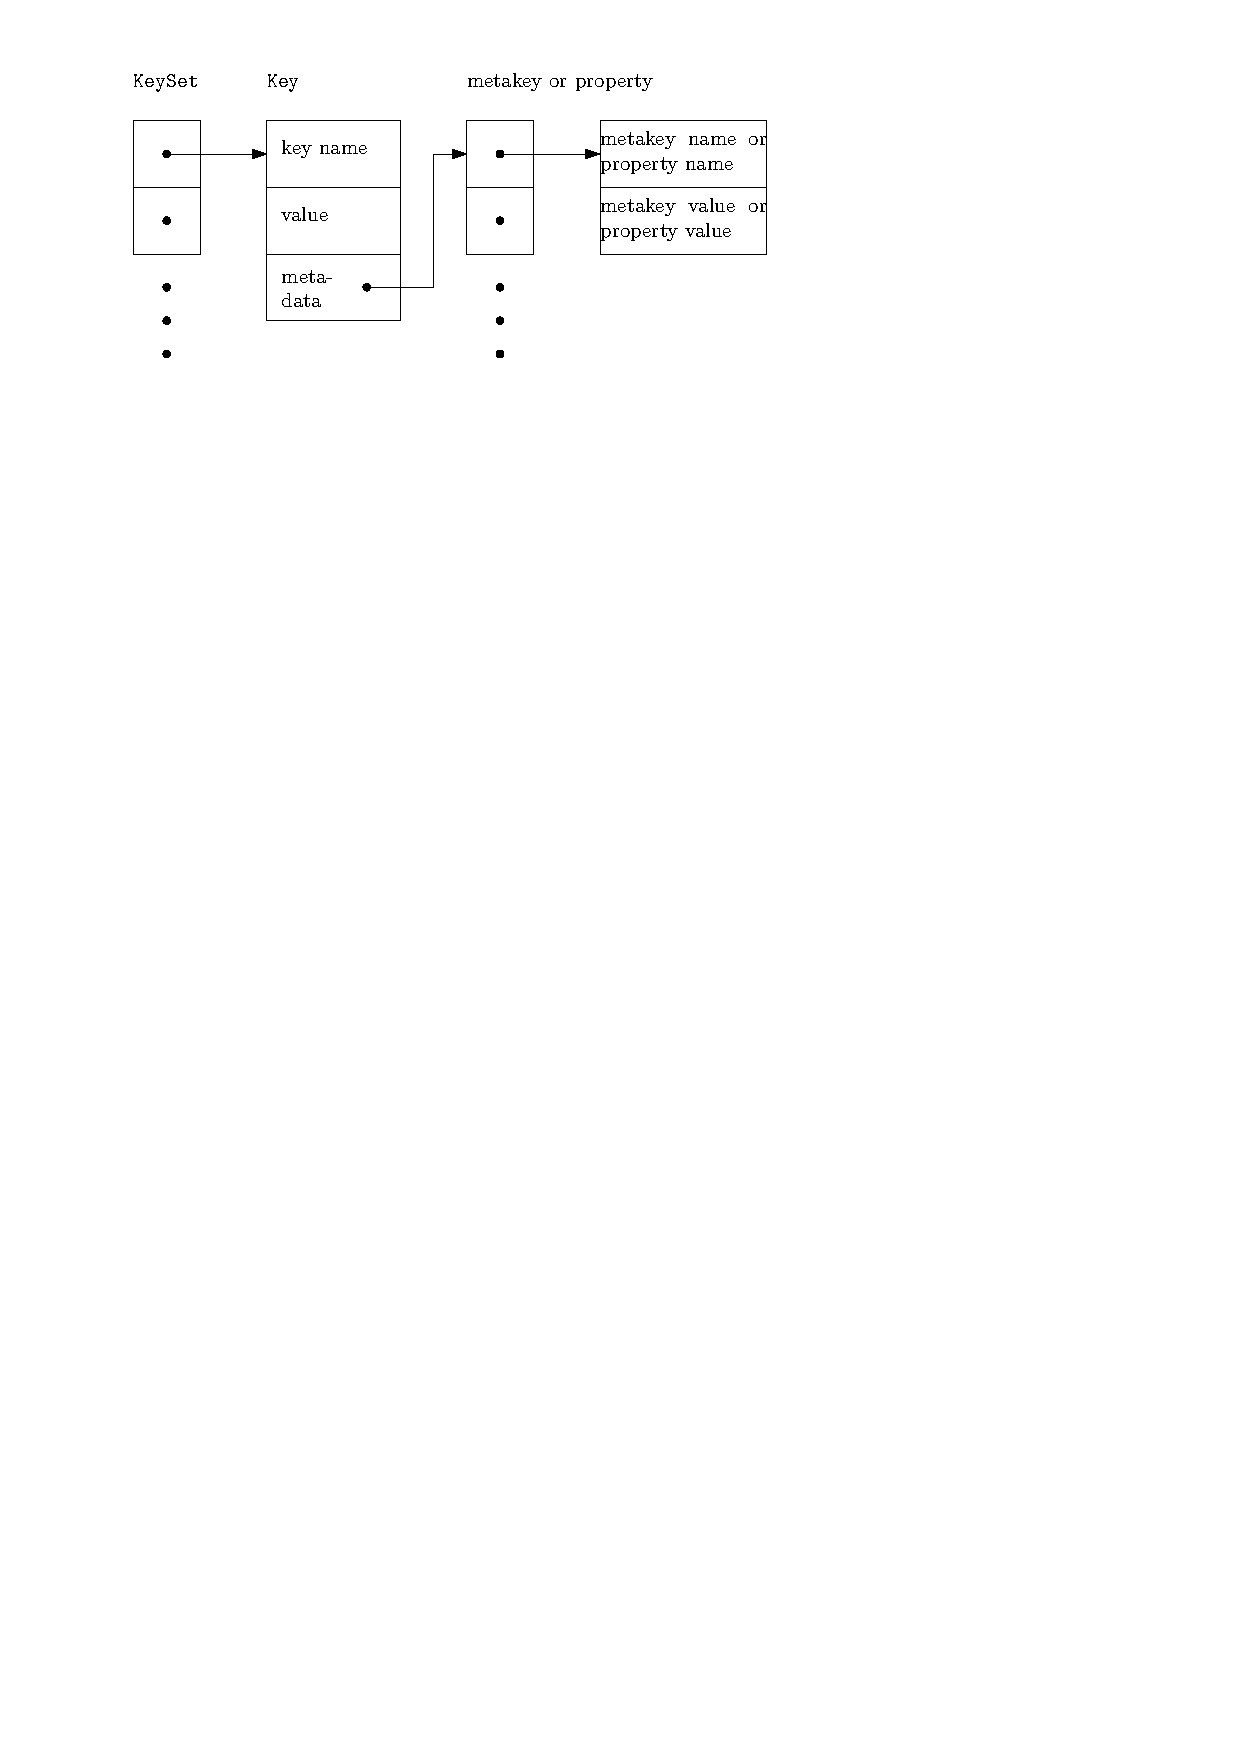
\includegraphics{keyset}
\end{frame}

\begin{frame}[fragile]
	\frametitle{KeySet Generation}
	\begin{alertblock}{Question}
	Idea: What if the configuration file format grammar describes source code?
	\end{alertblock}
	\pause

	\begin{grammar}
	<KeySet> ::= \lq ksNew'\WhiteSpace(' \{ <Key> \lq , \LineBreak'  \}  \{ \lq\WhiteSpace' \} \lq KS\_END);'

	<Key> ::= \lq keyNew \WhiteSpace ('' ' <key name> \lq ''  , \LineBreak' [ <Value> ] <properties> \lq KEY_END)'

	<Value> ::=  \{ \lq\WhiteSpace' \} \lq KEY\_VALUE, \WhiteSpace '' ' <configuration value> \lq ''  , \LineBreak'

	<properties> ::= \{ \{ \lq\WhiteSpace' \} <property> \lq , \LineBreak' \}

	<property> ::=  \lq KEY\_META, \WhiteSpace " ' <property name> \lq "  , \WhiteSpace " ' <property value> \lq " '
	\end{grammar}
\end{frame}

\begin{assignment}
	\begin{task}
	Break.
	\end{task}
\end{assignment}

\begin{frame}[fragile]
	\frametitle{Example}
	\begin{example}
	Given the key ^spec:/slapd/threads/listener^, with the configuration value ^4^ and the property $\property{default} \mapsto 1$, \elektra{Gen} emits:

	\begin{code}[gobble=4,language=Cpp]
	ksNew (keyNew ("spec:/slapd/threads/listener",
		       KEY_VALUE, "4",
		       KEY_META, "default", "1",
		       KEY_END),
	       KS_END);
	\end{code}
	\vspace{-1em}
	\end{example}

	\pause
	\begin{alertblock}{Finding}
	We have source code representing the settings.
	And if we instantiate it, we have a data structure representing the settings.
	Plugins emitting such ``configuration files'' are code generators.
	\end{alertblock}
\end{frame}

\begin{frame}[fragile]
	\frametitle{Implementation Strategies}

	\begin{itemize}
	\item Using ^print^ (only for very small generators)
	\item Using generative grammars
	\begin{code}[gobble=4,language=Cpp]
	query = '{' >> *(pair) > '}';
	pair = '{' >> key_name > '=' >> key_value >>
	       *('{' >> metakey_name > '=' >> metakey_value > '}')
	       > '}';
	\end{code}
	\item Using template languages (RubyERB, Cheetah, Mustache)
	\begin{code}[gobble=4,language=Python,basicstyle=\ttfamily\tiny,numberstyle=\ttfamily\tiny\color{blue}]
	@for n in hierarchy.name.split('/')[1:-1]
	namespace $support.nsnpretty($n)
	{
	class ${hierarchy.prettyclassname(support)}
	{
	typedef $support.typeof($hierarchy.info) type;
	@if $support.typeof($hierarchy.info) != "kdb::none_t"
	static type get(kdb::KeySet &ks, kdb::Key const& spec)
	{
		type value $support.valof($hierarchy.info)
		Key found(ckdb::ksLookup(ks.getKeySet(), *spec,
					ckdb::elektraLookupOptions::KDB_O_SPEC));
		return found.get<$support.typeof($hierarchy.info)>();
	}
	\end{code}
	\end{itemize}
\end{frame}

\begin{frame}
	\frametitle{Possible Properties}
	For example, SpecElektra has following properties:
	\begin{description}
	\item[type] represents the type to be used in the emitted source code.
	\item[opt] is used for short command-line options to be copied to the namespace \namespace{proc}.
	\item[opt/long] is used for long command-line options, which differ from short command-line options by supporting strings and not only characters.
	\item[readonly] yields compilation errors when developers assign a value to a contextual value within the program.
	\item[default] enables us to start the application even if the backend does not work.
	\end{description}
\end{frame}

\begin{frame}[fragile]
	With the specification:
	\par
	\begin{code}[gobble=4]
	[foo/bar]
	  default:=Hello
	  type:=string
	  opt:=b
	  readonly:=1
	\end{code}
	\par
	\elektra{Gen} gives the user read-only access to the object ^env.foo.bar^:
	\par
	\begin{code}[language=Cpp]
	std::cout << env.foo.bar;
	env.foo.bar = "Other world"; // comp. error
	\end{code}
	\par
	\small
	\pause
	Line~1 prints the configuration value of ^/foo/bar^ or ^"Hello"^ (without quotes) by default.
	When invoking the application with ^application -b "This world"^, the application would print ^"This world"^ (without quotes).
	Line~2 leads to a compilation error because of the property \property{readonly}.
\end{frame}

\begin{frame}[fragile]
	\frametitle{Which Configuration Access API?}

	First approach, one class (or function) per configuration setting:
	\\[1em]
	\begin{code}[gobble=4,language=Cpp]
	class SlapdThreadsListener : public Value<long,
		WritePolicyIs<ReadOnlyPolicy>> {
		... keyNew ("/slapd/threads/listener",
			    KEY_META, "type", "long",
			    KEY_META, "readonly", "1",
			    KEY_END) ...
	};
	\end{code}
\end{frame}

\begin{frame}[fragile]
	\frametitle{Which Configuration Access API?}

	Bad idea, manual instantiation and long names necessary:
	\\[1em]
	\begin{code}[gobble=4,language=Cpp]
	KeySet config;
	Context c;
	long foo ()
	{
		SlapdThreadsListener slapdThreadsListener (config, c);
		slapdThreadsListener++;
		return slapdThreadsListener;
	}
	\end{code}
\end{frame}

\begin{frame}[fragile]
	\frametitle{Which Configuration Access API?}

	Use hierarchy with namespaces or nested classes:
	\\[1em]
	\begin{code}[gobble=4,language=Cpp]
	namespace slapd
	{
	namespace threads
	{
	class Listener : public Value<long> {};
	}  // <continues on the next page>
	class Threads : public Value<none_t>
	{threads::Listener listener;};
	}  // end namespace slapd
	class Slapd : public Value<none_t>
	{slapd::Threads threads;};
	class Environment {Slapd slapd;};
	\end{code}
\end{frame}

\begin{frame}[fragile]
	\frametitle{Which Configuration Access API?}

	Much easier to use:
	\begin{code}[gobble=4,language=Cpp]
	long foo(slapd::Threads const & threads)
	{
		threads.listener++;
		Context & c = threads.context ();
		return threads.listener;
	}

	int main()
	{
		KeySet config;
		Context c;
		Environment env (config, c);
		long x = foo (env.slapd.threads);
	}
	\end{code}
\end{frame}

\begin{frame}[fragile]
	\frametitle{Which Configuration Access API?}

	In C, we use identifiers to be passed to the highlevel API\footnote{\url{https://www.libelektra.org/tutorials/high-level-api}}:
	\\[2em]
	\begin{code}[gobble=4,language=Cpp]
	elektraGetString (elektra, ELEKTRA_TAG_MY);
	\end{code}
	Where ^ELEKTRA_TAG_MY^ is a struct for that type.
	\\[2em]

	We can also omit the type:
	\begin{code}[gobble=4,language=Cpp]
	elektraGetLong (elektra, ELEKTRA_TAG_THREADS);
	elektraGet (elektra, ELEKTRA_TAG_THREADS);
	\end{code}
\end{frame}

\begin{frame}
	Guarantees by code generation:
	\begin{itemize}
	\item Every configuration setting is specified.
	\item (Data) type of source code and configuration settings match.
	\item Configuration access with defaults is always successful.
	Reason: We use defaults if everything else fails.
	\end{itemize}
	\vspace{3em}
	Missing Guarantee: Is every specified setting actually used?
\end{frame}



%%%%%%%%%%%%%%%%%%%%%%%%%%%%%%%%%%%%%%%%%% 
\section{Introspection vs. Generation}

\subsection{}

\begin{frame}
	\begin{alertblock}{Question}
	Introspection vs. Code Generation?
	\end{alertblock}
\end{frame}

\begin{frame}
	Limitations of introspection:
	\begin{itemize}
	\item no static checks
	\item no whole-program optimizations (API barriers)
	\end{itemize}
\end{frame}

\begin{frame}
	Overhead without code generation (=backend) is $1.8$x higher~\cite{raab2015kps}:
	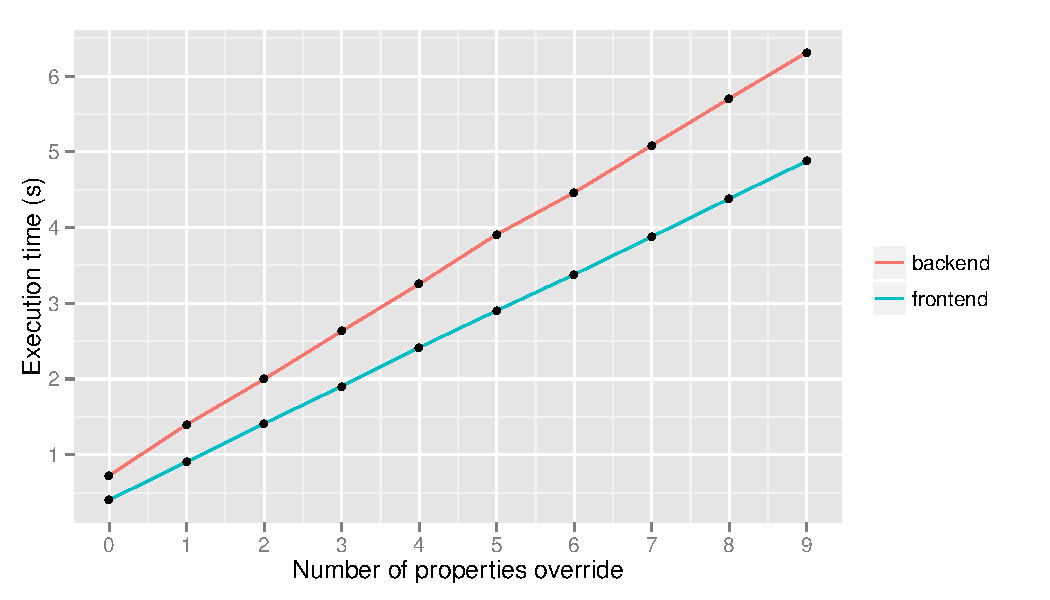
\includegraphics[width=\textwidth]{mean2}
\end{frame}

\begin{frame}
	But it might not matter because configuration access might not be a bottleneck~\cite{raab2015kps},
	for example, a word counting application:

	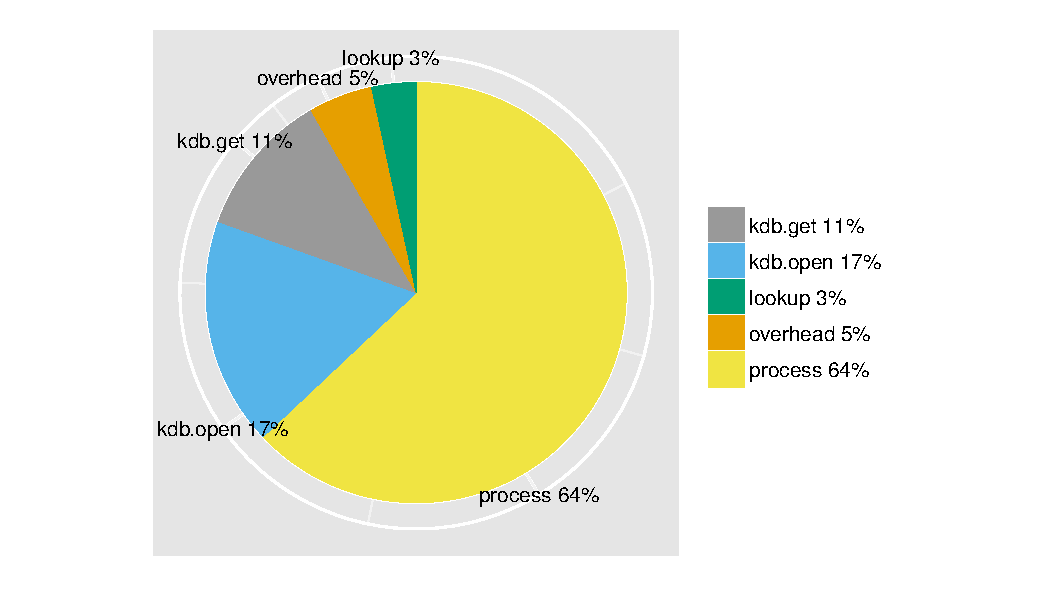
\includegraphics[width=\textwidth]{wc}

	But: \pause
	Configuration access points within loops might be a bottleneck.
\end{frame}

\begin{frame}
	Advantages of introspection:
	\pause
	\begin{itemize}
	\item specification can be updated live on the system without recompilation
	\item tooling has generic access to all specifications
 	\item new features the key database (e.g., better validation) are immediately available consistently
	\end{itemize}
	\vspace{1em}
	\begin{alertblock}{Implication}
	We generally prefer introspection, except for a very thin configuration access API.
	\end{alertblock}
	\vspace{1em}
	\begin{restatable}{requirement}{reqIntrospection}
	Configuration settings and specifications must be introspectable.%
	\end{restatable}
\end{frame}

\begin{frame}
	\frametitle{Preview}
	\begin{itemize}
	\item Testing
	\item Early Detection of Misconfiguration
	\end{itemize}
\end{frame}



%%%%%%%%%%%%%%%%%%%%%%%%%%%%%%%%%%%%%%%%%% 
\nocite{raab2017introducing}

\appendix

\begin{frame}[allowframebreaks]
	\bibliographystyle{plainnat}
	\bibliography{../shared/elektra.bib}
\end{frame}

\end{document}


